\subsection{\large{Расчётная модель данных}}
\addcontentsline{toc}{subsection}{Расчётная модель данных}

Так как генплан состоит из большого количества разнородных объектов,
то необходимо предусмотреть легко расширяемую и понятную модель данных,
которая будет удобна в использовании исследователям и аналитикам.
Для генплана используются следующие объекты:
\begin{itemize}
    \item допустимая для строительства область на карте;
    \item стоимостная модель расчета стоимости инженерной подготовки;
    \item перечень сооружений с указанием габаритов (ширина, длина, радиус),
    степени огнестойкости, категории взрывопожарной и пожарной опасности, конструктивной пожарной опасности;
    \item параметры коммуникаций между сооружениями проектируемого объекта;
    \item зоны распространения теплового потока;
    \item зоны распространения взрывной волны;
	\item и т.д.
\end{itemize}

Для решения поставленной задачи предлагается следующая расчётная модель данных, изображенная
на верхнеуровневой диаграмме классов
Основная цель создания этой модели данных -- это снижение издержек на обмен данными между
сервисами расчётного модуля.
В силу сложности предметной области и большого количества технической терминологии,
критерий понятности чрезвычайно важен.

Ниже представлена верхнеуровневая диаграмма классов расчётной модели данных
(см. рис\ \ref{pic:architecture__model-classes}).

\begin{figure}[H]
	\hspace*{-2.5 cm}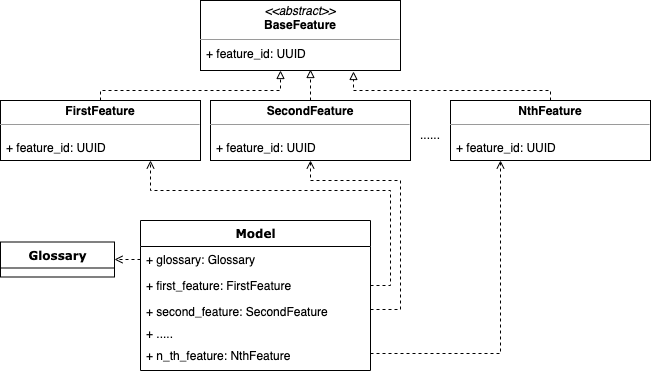
\includegraphics[width=0.7\textwidth, left]{architecture/pictures/model/classes}
	\caption{Верхнеуровневая диаграмма классов расчётной модели данных}
	\label{pic:architecture__model-classes}
\end{figure}
\vskip 5 mm

Расчётная модель данных представлена следующими классами.
\begin{itemize}
	\item \textbf{Model} -- верхнеуровневый класс, который и является расчётной моделью данных, использующийся
	при передаче данных между сервисами. Состоит из расчётных элементов и глобального регистра типов объектов.
	\item {
		\textbf{Feature} -- расчётный элемент. Являются составными частями расчётной модели данных. Например, расчётными
		элементами являются местоположения сооружений, внутриплощадочные проезды и т.д.
	}
	\item {
		\textbf{Glossary} -- объект, являющийся глобальным перечнем типов различных объектов.
		Например, типы сооружений, такие как "Сепаратор", "Трансформаторная подстанция", "Насосная" хранятся именно
		здесь. Помимо описания типа, именно здесь хранятся его различные характеристики. Для типа "Электрокабель 35 кВ"
		определены параметра диаметра сечения, удельного сопротивления и используемого материала.
	}
\end{itemize}